\section{Aufgabe 5 - Ansteuerung eines Lautsprechers}
\label{sec:aufgabe-5---ansteuerung-eines-lautsprechers}

In dieser Aufgabe wird ein 4 Bit großes Signal, mittels einer Schaltung, in ein analoges Signal umgewandelt.
Dieses Signal soll dann auf einem Lautsprecher ausgegeben werden.

Die Umwandlung von einem digitalen Signal zu einem Analogen geschieht mithilfe eines sogenannten R2R-Netzwerk.
Dieses addiert das Signal eines Bits proportional zu dessen Position zum anaolgen Signal.
Das resultierende Signal wird dann durch einen Operationsverstärker soweit verstärkt, dass es hörbar an einem Lautsprecher ausgegeben werden kann.

Ein R2R-Netzwerk ist eine Schaltung aus Widerständen welche jeweils die Größe $R$ und $2R$ besitzen.
Ein Beispiel dieser Schaltung befindet sich im Abschnitt \ref{subsec:a5-vorbereitung} und wird auch in der Praktikumsaufgabe implementiert.

\subsection{Materialien}
\label{subsec:a5-materialien}

\begin{table}[h]
    \centering
    \caption{Aufgabe 5 - Verwendete Materialien}
    \label{tab:a5-materialien}
    \begin{tabular}{| l | l | l |}
        \hline
        Bezeichnung & Eigenschaften & Menge \\
        \hline
        Widerstand  & $100k\Omega$   & 5     \\
        & Braun - Schwarz - Gelb - Gold & \\
        Widerstand  & $51k\Omega$   & 3   \\
        & Grün - Braun - Orange - Gold & \\
        Widerstand  & $3k\Omega$   & 1   \\
        & Orange - Schwarz - Rot - Gold  & \\
        Kondensator & $10\mu F$ 1 \\
        Operationsverstärker & MCP6241 & 1 \\
        Lautsprecher & k.A. & 1 \\
        Mikrocontroller & Arduino Uno R3 & 1 \\
        \hline
    \end{tabular}
\end{table}

\newpage

\subsection{Vorbereitung}
\label{subsec:a5-vorbereitung}

\subsubsection{Aufgabe 1}
In Abbildung \ref{fig:gegebene-r2r-schaltung} ist das gegebene R2R-Netzwerk zu sehen.

\begin{figure}
    \centering
    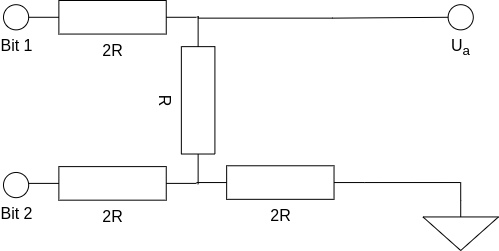
\includegraphics[width=\textwidth]{pictures/a5-1-vorbereitung.png}
    \caption{Gegebene R2R-Schaltung}
    \label{fig:gegebene-r2r-schaltung}
\end{figure}

\textbf{a,b)} Es sind die Werte für $U_a$ allgemein zu berechnen, unter der Annahme der folgenden Werte für $U_{Bit 1}$ und $U_{Bit 2}$.

\begin{tabular}{| l | l |}
    \hline
    $U_{Bit 1}$ & $U_{Bit 2}$ \\
    \hline
    $0V$ & $0V$ \\
    $0V$ & $U_{Bit}$ \\
    $U_{Bit}$ & $0V$ \\
    $U_{Bit}$ & $U_{Bit}$ \\
    \hline
\end{tabular}

Um die Werte für $U_a$ zu berechnen, ist es am besten, zuerst die allgemeine Formel, die in \textbf{b)} gesucht wird zu finden, um dann einzusetzen.
Da $U_{Bit 1}$ und $U_{Bit 2}$ als Spannungsquellen betrachtet werden können, kann mittels dem Überlagerungssatz von Helmholz eine allgemeine Formel gefunden werden.

\textbf{Fall 1} - $U_{Bit 2}$ wird kurzgeschlossen:

Es resultiert das Schaltbild von Abbildung \ref{fig:fall-1}.
\begin{figure}[h]
    \centering
    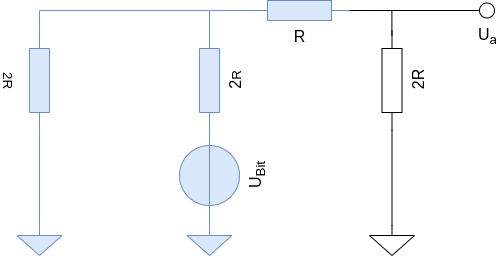
\includegraphics[width=\textwidth]{pictures/a5-1-fall-1.png}
    \caption{Fall 1}
    \label{fig:fall-1}
\end{figure}

\newpage

Die mit Blau markierten Komponenten können  zu einer Schaltung mit einer Ersatzspannungsquelle mit Innenwiderstand zusammengefasst werden.
Der Innenwiderstand beträgt demnach:

\begin{align}
    R_i = 2R || 2R + R \\
    = 2R
\end{align}

Da bei eine Leerlaufspannung die Klemmen offen sind, wird der Widerstand $R$ effektiv kurzegschlossen.
Der Leerlaufwiderstand is daher der Spannungsabfall über den Widerstand $2R$:

\begin{align}
    U_L = U_{2R} \\
    = I * 2R \\
    = \frac{U_{Bit}*2R}{R_g} \\
    = \frac{U_{Bit}*2R}{2R + 2R} \\
    = \frac{U_{Bit}}{2} \\
\end{align}

Die Resultierende Spannung $U_{a1}$ ist dann gleich der Spannung über den nicht in der Ersatzspannungsquelle inkludierten Widerstands $2R$:

\begin{align}
    U_{a1} = I * 2R \\
    = \frac{U_L * 2R}{R_i + 2R} \\
    = \frac{\frac{U_{Bit}}{2} * 2R}{2R + 2R} \\
    = \frac{U_{Bit}R}{4R} \Rightarrow\\
    \underline{\underline{U_{a1} = \frac{U_{Bit}}{4}}}
\end{align}

\textbf{Fall 2} - $U_{Bit 1}$ wird kurzgeschlossen:

Es resultiert das Schaltbild von Abbildung \ref{fig:fall-2}.
\begin{figure}[h]
    \centering
    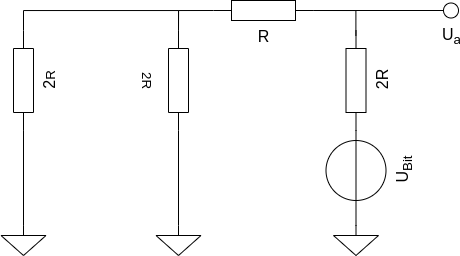
\includegraphics[width=\textwidth]{pictures/a5-1-fall-2.png}
    \caption{Fall 2}
    \label{fig:fall-2}
\end{figure}

Die linken Widerstände können zusammengefasst werden zu $2R || 2R = R$
Es folgt:

\begin{align}
    U_{a2} = U_{Bit} - U_{2R} \\
    = U_{Bit} - \frac{U_{Bit}}{R_g} * U_{2R} \\
    = U_{Bit} - \frac{U_{Bit} * 2R}{4R} \\
    = \frac{U_{Bit}}{2}
\end{align}

Aus Fall 1 und Fall 2 folgt nun die Lösung für \textbf{b)}:

\begin{align}
    U_a = U_{a1} + U_{a2} \\
    =  \frac{U_{Bit}}{2} +  \frac{U_{Bit}}{4} \Rightarrow
\end{align}

Man kann erkennen, dass die Spannung für jedes Bit halbiert wird.
D.h., die Gewichtung eines Bits ist $\frac{Bit_n}{Bit_{n-1}} = \frac{1}{2}$
Daraus folgt die Formel:

\begin{align}
    U_{a(1\dots n)} = \sum_{k=1}^{n}  \frac{U_{Bit}}{2^n}
\end{align}

Es folgt daraus die folgende Wertetabelle für \textbf{a)}

\begin{tabular}{| l | l | l |}
    \hline
    $U_{Bit 1}$ & $U_{Bit 2}$ & $U_a$ \\
    \hline
    $0V$ & $0V$ & $0V$ \\
    $0V$ & $U_{Bit}$ & $\frac{U_{Bit}}{4}$\\
    $U_{Bit}$ & $0V$  & $\frac{U_{Bit}}{2}$ \\
    $U_{Bit}$ & $U_{Bit}$  & $\frac{3}{4}U_{Bit}$\\
    \hline
\end{tabular}

\textbf{c)} Es ist die Berechnungsvorschrift auf ein 4-Bit R2R Netzwerk anzuwenden:

\begin{align}
    U_{a(1_4)} = \frac{U_{Bit}}{2} + \frac{U_{Bit}}{4} + \frac{U_{Bit}}{8} + \frac{U_{Bit}}{16} \\
    =  \frac{8U_{Bit}}{16} + \frac{4U_{Bit}}{16} + \frac{2U_{Bit}}{16} + \frac{U_{Bit}}{16} \\
    =  \frac{15U_{Bit}}{16}
\end{align}

\subsubsection{Aufgabe 2}

Es ist zu Berechnen, welche Werte ausgegeben werden, damit ein gegebenes Ausganssignal erreicht wird.
Für die Ausgabe gibt es 16 verschiedene Werte.
Je niedriger der Wert, desto niedriger ist die resultierende Ausgangsspannung.
Zur Berechnung wird daher folgende Formel verwendet.
Da eine Ganzzahl benötigt wird werden die Ergebnisse gerundet.

\begin{align}
    n = 5 / 16 * U_{sin}
\end{align}


\begin{table}[h]
    \centering
    \caption{Zuordnung der Spannungswerte}
    \label{tab:zuordnung-der-spannungswerte}
    \begin{tabular}{| c | c | c |}
        \hline
        $U_{sin}$ & Dezimal & Hexadezimal \\
        \hline
        $2,3$ & $7$ & $1$ \\
        $3,0$ & $9$ & $5$ \\
        $3,7$ & $11$ & $3$ \\
        $4,2$ & $13$ & $7$ \\
        $4,6$ & $14$ & F \\
        $4,7$ & $15$ & $7$ \\
        $4,6$ & $14$ & F \\
        $4,2$ & $13$ & $7$ \\
        $3,7$ & $11$ & $3$ \\
        $3,0$ & $9$ & $5$ \\
        $2,3$ & $7$ & $1$ \\
        $1,6$ & $5$ & $5$ \\
        $1,0$ & $3$ & $3$ \\
        $0,4$ & $1$ & $1$ \\
        $0,1$ & $0$ & $0$ \\
        $0,0$ & $0$ & $0$ \\
        $0,1$ & $0$ & $0$ \\
        $0,4$ & $1$ & $1$ \\
        $1,0$ & $3$ & $3$ \\
        $1,6$ & $5$ & $5$ \\
        \hline
    \end{tabular}
\end{table}

\newpage

\subsubsection{Aufgabe 3}

Es soll für bestimmte Frequenzen berechnet werden, wielange ein Bitmuster anliegen muss.
Dafür ist die Frequenz in Hz gegeben und es werden laut Angabe 20 Bitmuster pro Signalperiode benötigt.
Da die Frequenz der Kehrwert der Zeit pro Signalperiode ist, kann folgende Formel zu berechnung der gesuchten Zeit verwendet werden.

\begin{align}
    n = \frac{\frac{1}{frequenz}}{20}
\end{align}

Damit ergiben sich folgende Werte für bestimmte Frequenzen.

\begin{table}[h]
    \centering
    \caption{Zeit pro Bitmuster}
    \label{tab:zeit-pro-bitmuster}
    \begin{tabular}{| c | c | c |}
        \hline
        Ton & Frequenz (Hz) & Zeit pro Bitmuster ($\mu s$) \\
        \hline
        c' & $262$ & $190,84$ \\
        d' & $294$ & $170,068$ \\
        e' & $330$ & $151,\overline{51}$ \\
        f' & $349$ & $143,266$ \\
        g' & $392$ & $127,5\overline{51}$ \\
        a' & $440$ & $113,\overline{63}$ \\
        h' & $494$ & $101,215$ \\
        \hline
    \end{tabular}
\end{table}

\subsection{Praktikumsaufgabe}
\label{subsec:a5-praktikumsaufgabe}

Es wurde die Schaltung implementiert aus Abbildung \ref{fig:a5-praktik} implementiert.
Nach dem besprochenen R2R-Netzwerk, welches die Pins 7, 6, 5 und 4 als Eingabe hat, folgt die Verstärkung des Signals über einen Operationsverstärker.
Da der Operationsverstärker Signale zwischen 0V und 5V erzeugt, der Lautsprecher jedoch eine Spannung von $-2,5V \leq U \leq 2,5V$ benötigt folgt ein Kondensator, welche die Spannung zentiert.
Der darauf folgende Widerstand regelt die Lautstärke des Tons.
Der Widerstand kann daher beliebig gewählt werden, je nach Vorlieben für verschiedene Lautstärken.

Das Programm soll weiters ein Klavier implementieren.
D.h., bei Eingabe der Tasten ’’a’’, ’’s’’, ’’d’’, ’’f’’, ’’g’’, ’’h’’, ’’j’’ sollen jeweils die Töne ’’c'’’, ’’d'’’, ’’e'’’, ’’f'’’, ’’g'’’, ’’a'’’, ’’h''' ausgegeben werden.
Um die benötigte Geschwindigkeit beim Schalten der Pins zu erreichen, werden die Register die diese verwalten direkt angesprochen.

\begin{figure}[h]
    \centering
    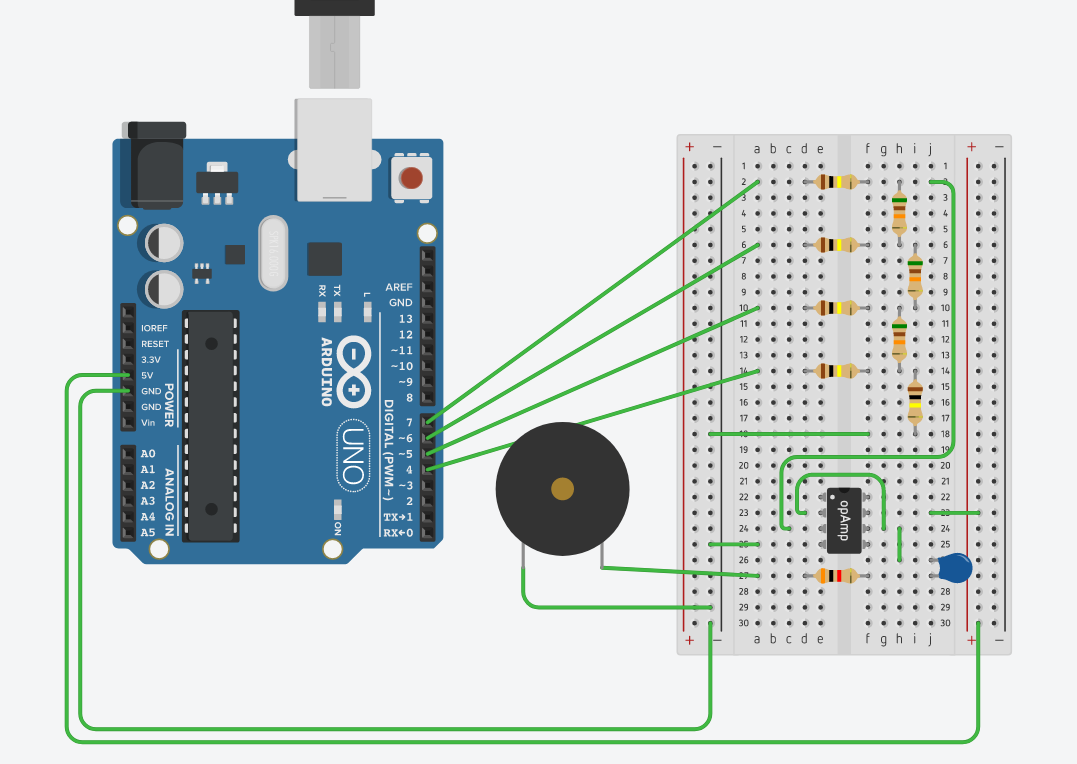
\includegraphics[width=\textwidth]{pictures/a5-praktik.png}
    \caption{Implementierte Schaltung aus Aufgabe 5}
    \label{fig:a5-praktik}
\end{figure}

Im nachfolgenden Text wird der Programmcode der Aufgabe erläutert.
Einzelne Teile des Codes werden ausgewählt und beschrieben.
Am Ende dieser Sektion befindet sich der vollständige Programmcode.

\begin{lstlisting}[language=C,label={lst:a5-anlegen-der-pins}, caption={Anlegen der Pins über Register}]
void setup()
{
    Serial.begin(9600);

    DDRD = DDRD | B11111100;
}
\end{lstlisting}

\newpage

In Listing \ref{lst:a5-anlegen-der-pins} werden die benötigten Pins konfiguriert.
Das Register ''DDRD'' verwaltet die Pins 0 bis 7.
Durch das übergebene Bitmuster, werden die Pins 7 bis 2 als Ausgabepins konfiguriert.
Konfiguration über die Methode $pinMode()$ ist nicht mehr nötig.
Des weiteren ist das Einstellen der Pins 2 und 3 ein Artifakt des Debuggens des Programms und ist nicht notwendig.

\begin{lstlisting}[language=C,label={lst:a5-lesen-von-eingaben}, caption={Lesen von Eingaben}]
void loop()
{
    double time = (double)millis() / 1000;

    if (Serial.available() > 0) {
        last_read = Serial.read();
    }
    ...
}
\end{lstlisting}

\newpage

Listing \ref{lst:a5-lesen-von-eingaben} zeigt, wie Eingaben des Benutzers eingelesen werden können.
Durch das Aufrufen von $Serial.available()$ wird abgefragt, ob eine Eingabe getätigt wurde.
$Serial.read()$ speichert die Eingabe dann in einer globalen Variable.

\begin{lstlisting}[language=C,label={lst:a5-eingabe-pruefen}, caption={Prüfen von Eingaben}]
    switch(last_read) {
        case A:
            play_frequency(NOTE_C, time);
        break;
        case S:
            play_frequency(NOTE_D, time);
        break;
        case D:
            play_frequency(NOTE_E, time);
        break;
        case F:
            play_frequency(NOTE_F, time);
        break;
        case G:
            play_frequency(NOTE_G, time);
        break;
        case H:
            play_frequency(NOTE_A, time);
        break;
        case J:
            play_frequency(NOTE_H, time);
        break;
        default:
            PORTD = B00000000;
        break;
    }
}
\end{lstlisting}

Benutzereingaben von Listing \ref{lst:a5-lesen-von-eingaben} wird hier, in Listing \ref{lst:a5-eingabe-pruefen}, überprüft.
Die Konstanten die hier verwendet werden, sind den ASCII-Werten der jeweiligen Buchstaben zugeordnet.
Dies hat zur Folge, dass nur Kleinbuchstaben als korrekte Eingaben erkannt werden.
Wird eine Eingabe nicht erkannt, werden die Pins mittels dem Register $PORTD$ ausgeschaltet.
$PORTD$ ist ein Register, ähnlich wie $DDRD$, welches die Ausgabe der Pins von 7 bis 0 steuert.

\newpage

\begin{lstlisting}[language=C,label={lst:a5-play-frequency}, caption={Abspielen von Frequenzen}]
void play_frequency(int frequency, double time) {
    //sin is from -1 to 1 so +1 to start at 0
    double y = sin(frequency * time) + 1;
    byte value = y / 2 * 16;
    PORTD = value << 2;
}
\end{lstlisting}

Die Methode $playFrequency(\dots)$ aus Listing \ref{lst:a5-play-frequency} spielt schließlich den Ton ab.
Sie übernimmt eine gewünschte Frequenz, sowie die Zeit, welche seit dem Programmstart vergangen ist.
Durch das Aufrufen von $\sin(...)$ mit den genannten Variablen wird ein Wert für das Sinussignal berechnet.
Dieser Wert ist $-1 \leq n \leq 1$ und muss daher mittels der Addition von 1 auf  $0 \leq n \leq 2$ gebracht werden, um ihn anschließend auf $0 \leq n \leq 1$ zu normalisieren.
Mittels der Multiplikation mit 16 wird der Wert errechnet, welcher laut Vorbereitung benötigt wird.
Durch das Bitshifting in der letzten Zeile, um zwei Bitstellen, werden die entsprechenden Pins geschaltet.

\begin{lstlisting}[language=C,label={lst:a5-programmcode}, caption={Vollständiger Programmcode der Aufgabe 5}]
#include <math.h>

const int PIN_1 = 7;
const int PIN_2 = 6;
const int PIN_3 = 5;
const int PIN_4 = 4;

const int FREQUENCY = 440;

const int NOTE_C = 262;
const int NOTE_D = 294;
const int NOTE_E = 330;
const int NOTE_F = 349;
const int NOTE_G = 392;
const int NOTE_A = 440;
const int NOTE_H = 494;

const int A = 'a';
const int S = 's';
const int D = 'd';
const int F = 'f';
const int G = 'g';
const int H = 'h';
const int J = 'j';

double previous_time = 0;

int last_read = 97;

void setup()
{
  Serial.begin(9600);

  DDRD = DDRD | B11111100;
}

void loop()
{
  double time = (double)millis() / 1000;

  if (Serial.available() > 0) {
    last_read = Serial.read();
  }

  switch(last_read) {
    case A:
    	play_frequency(NOTE_C, time);
    break;
    case S:
    	play_frequency(NOTE_D, time);
    break;
    case D:
    	play_frequency(NOTE_E, time);
    break;
    case F:
    	play_frequency(NOTE_F, time);
    break;
    case G:
    	play_frequency(NOTE_G, time);
    break;
    case H:
    	play_frequency(NOTE_A, time);
    break;
    case J:
    	play_frequency(NOTE_H, time);
    break;
    default:
    	PORTD = B00000000;
    break;
  }
}

void play_frequency(int frequency, double time) {

  //sin is from -1 to 1 so +1 to start at 0
  double y = sin(frequency * time) + 1;
  byte value = y / 2 * 16;
  PORTD = value << 2;
}
\end{lstlisting}

\subsection{Fehlerdiskussion}
\label{subsec:a5-fehlerdiskussion}

In der Methode $play_frequency$ werden die falschen Pins angesprochen.
Die Bits der $value$ Variable müssten um 4 Stellen verschoben werden anstelle von 2.
Die Werte von 0 bis 16 werden mittels 4 Bits abgebildet, während in dem Register 8 Bits vorhanden sind.
In der derzeitigen Implementierung werden maximal die Pins 5 und 4 angesprochen, nicht jedoch 7 und 6.
Mittels eines Shifts um 4 anstelle von 2 können alle benötigten Pins angesprochen werden.
